%%%%%%%%%%%%%%%%%%%%%%%%%%%%%%%%%%%%%%%%%%%%%%%%%%%%%%%%%%%%%%%%%%%%%%%%%%%%%%%%
\begin{frame}{MPI}
	\Large{\highlightB{MPI - Message Passing Interface}}
	\normalsize
	
	\begin{itemize}
		\item A standard for a library interface for parallel programs.
		\item \highlight{process-based}: interface to send message from one process to another process.
		\item  \highlight{distributed memory}: every memory has its own virtual memory.
	\end{itemize}
	\centering
	
	\tikzset{
		main/.style={black, line width=0.4mm, opacity=1},
		second/.style={gray, opacity=5},
		arrow/.style={-latex, shorten >=1ex, shorten <=1ex, bend angle=45}
	}
	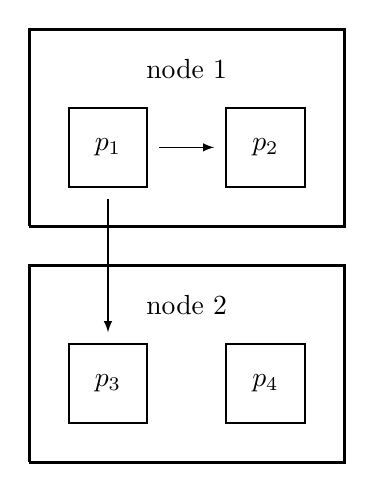
\begin{tikzpicture}
	
	
	\draw[main] (0,0) -- (4,0) -- (4,2.5)-- (0,2.5)-- (0,0);
	
	\node (rect) at (1,1) [draw,thick,minimum width=1cm,minimum height=1cm]  {$p_3$};
	\node (rect) at (3,1) [draw,thick,minimum width=1cm,minimum height=1cm]  {$p_4$};
	
	\draw[main] (0,3) -- (4,3) -- (4,5.5)-- (0,5.5)-- (0,3);
	
	\node (rect) at (1,4) [draw,thick,minimum width=1cm,minimum height=1cm]  {$p_1$};
	\node (rect) at (3,4) [draw,thick,minimum width=1cm,minimum height=1cm]  {$p_2$};
	
	\draw [arrow]  (1.5,4) to (2.5,4);
	\draw [arrow]  (1,3.5) to (1,1.5);
	
	\node at (2,5) {node 1};
	\node at (2,2) {node 2};	
	
	\end{tikzpicture}



\end{frame}

%%%%%%%%%%%%%%%%%%%%%%%%%%%%%%%%%%%%%%%%%%%%%%%%%%%%%%%%%%%%%%%%%%%%%%%%%%%%%%%%
\begin{frame}{MPI}
	\Large{\highlightB{MPI\_Bcast}}
	\normalsize
	
	\centering
	\vspace{1cm}
	\tikzset{
	main/.style={black, line width=0.4mm, opacity=1},
	second/.style={gray, opacity=5},
	arrow/.style={-latex, shorten >=1ex, shorten <=1ex, bend angle=45}
}
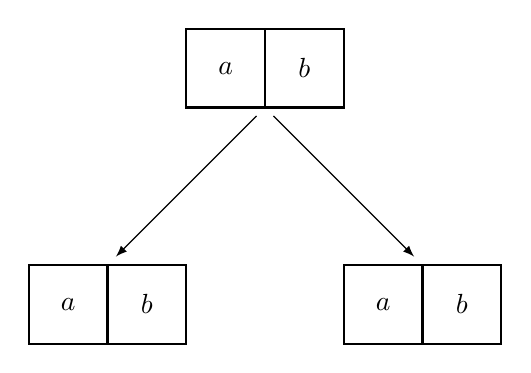
\begin{tikzpicture}

\node (rect) at (2,0) [draw,thick,minimum width=1cm,minimum height=1cm]  {$a$};
\node (rect) at (3,0) [draw,thick,minimum width=1cm,minimum height=1cm]  {$b$};

\node (rect) at (0,-3) [draw,thick,minimum width=1cm,minimum height=1cm] {$a$};
\node (rect) at (1,-3) [draw,thick,minimum width=1cm,minimum height=1cm] {$b$};

\node (rect) at (4,-3) [draw,thick,minimum width=1cm,minimum height=1cm] {$a$};
\node (rect) at (5,-3) [draw,thick,minimum width=1cm,minimum height=1cm] {$b$};


\draw [arrow]  (2.5,-0.5) to (0.5,-2.5);
\draw [arrow]  (2.5,-0.5) to (4.5,-2.5);

\end{tikzpicture}
		
\end{frame}

%%%%%%%%%%%%%%%%%%%%%%%%%%%%%%%%%%%%%%%%%%%%%%%%%%%%%%%%%%%%%%%%%%%%%%%%%%%%%%%%
\begin{frame}{MPI}
	\Large{\highlightB{MPI\_Reduce with MPI\_sum}}
	\normalsize
	
	\centering
	\vspace{1cm}
	\tikzset{
	main/.style={black, line width=0.4mm, opacity=1},
	second/.style={gray, opacity=5},
	arrow/.style={-latex, shorten >=1ex, shorten <=1ex, bend angle=45}
}
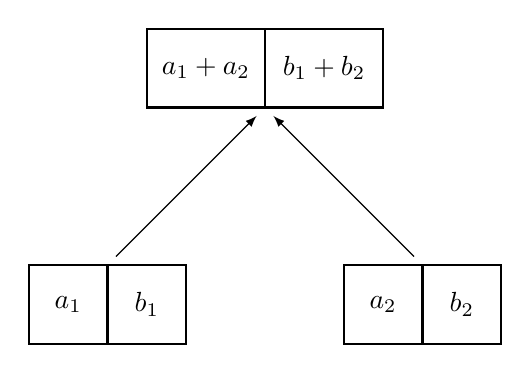
\begin{tikzpicture}

\node (rect) at (1.75,0) [draw,thick,minimum width=1.5cm,minimum height=1cm] {$a_1 + a_2$};
\node (rect) at (3.25,0) [draw,thick,minimum width=1.5cm,minimum height=1cm] {$b_1 + b_2$};


\node (rect) at (0,-3) [draw,thick,minimum width=1cm,minimum height=1cm] {$a_1$};
\node (rect) at (1,-3) [draw,thick,minimum width=1cm,minimum height=1cm] {$b_1$};


\node (rect) at (4,-3) [draw,thick,minimum width=1cm,minimum height=1cm] {$a_2$};
\node (rect) at (5,-3) [draw,thick,minimum width=1cm,minimum height=1cm] {$b_2$};


\draw [arrow]  (0.5,-2.5) to (2.5,-0.5) ;
\draw [arrow]  (4.5,-2.5) to (2.5,-0.5) ;

\end{tikzpicture}
	
\end{frame}

